\section{Methodology}

To effectively report the trends in how contextual features predict LSA outcomes, the educational production function framework \cite{bowles1970towards} and repeated cross-sectional analysis \cite{Buck1995ChoosingIssues} were utilized.


To effectively report the trends in how contextual features predict LSA outcomes, this chapter utilizes the educational production function framework \cite{bowles1970towards} and conducted a repeated cross-sectional analysis \cite{Buck1995ChoosingIssues}. This analysis was guided by the well-established Cross-Industry Standard Process for Data Mining (CRISP-DM) \cite{chapman1999cross}and complemented by the Domain-Driven Data Mining (D$^3$M) approach \cite{Cao2005DomainMethodology, Cao2009IntroductionMining}. This process involves multiple phases integral to the. Here, domain knowledge plays a pivotal role throughout, ensuring that the developed models are not only statistically sound with a good predictive performance, but also actionable and relevant in real-world applications.

\begin{figure}[ht!]
\centering
\caption{\textmd{The case-study methodology}}
\label{fig:process}
\fcolorbox{gray}{white}{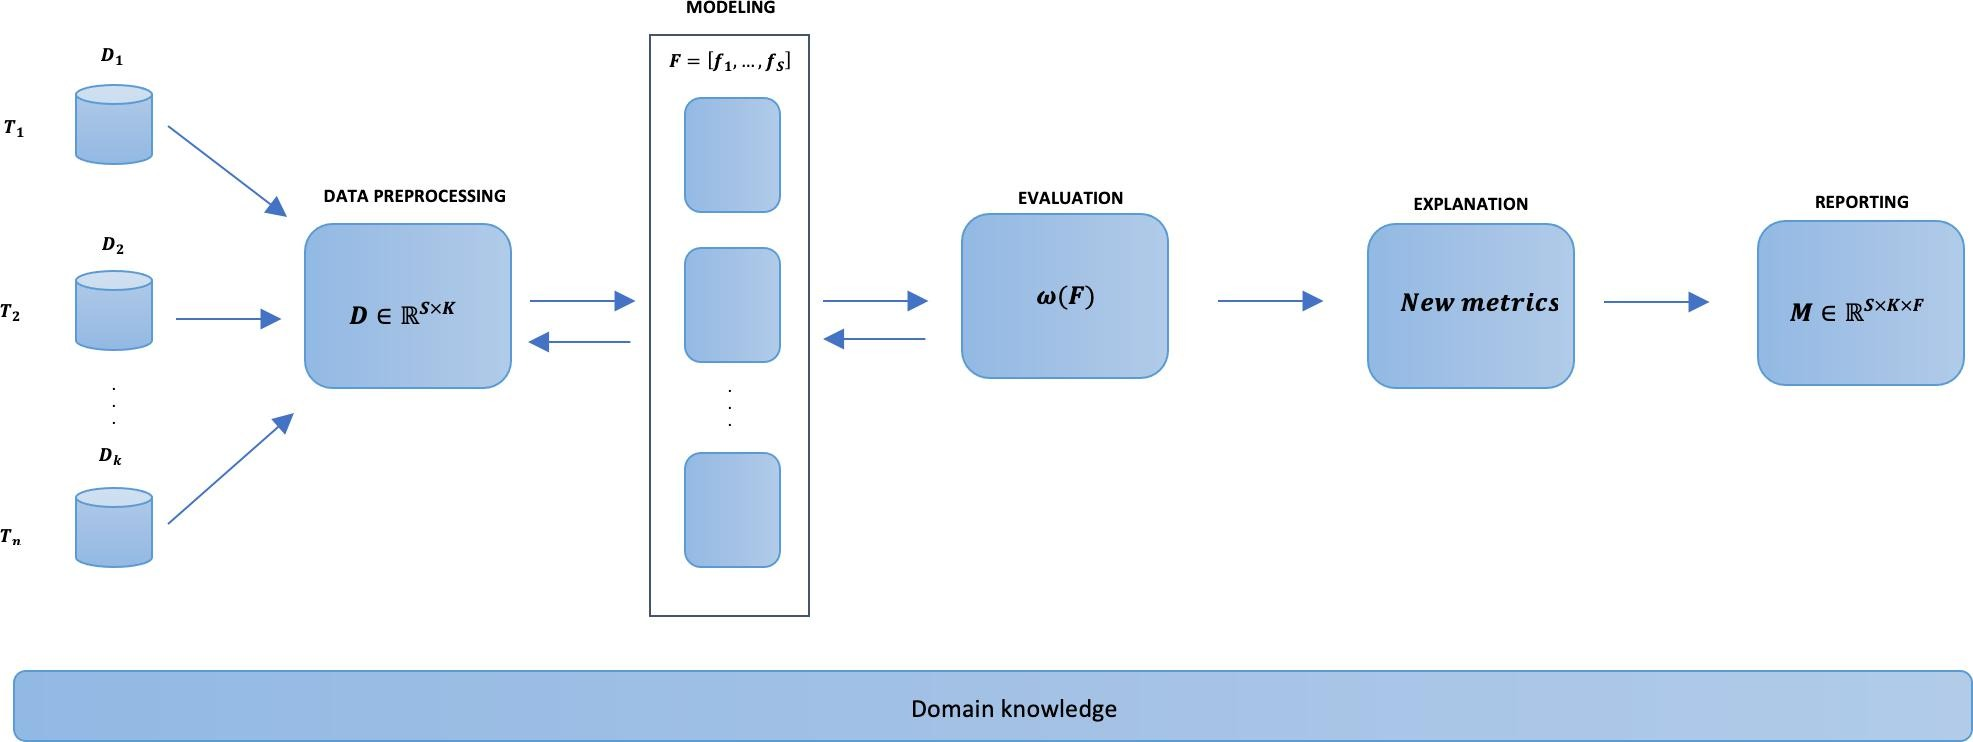
\includegraphics[width=0.9\textwidth]{images/realApplication/framework.jpg}}
\par\medskip\ABNTEXfontereduzida\selectfont\textbf{source: self-provided} \par\medskip
\end{figure}

Figure \ref{fig:process} outlines the case-study methodology. Specifically, consider a dataset \( D = [d_1, \ldots, d_k] \) with contextual features \( X = [x_1, \ldots, x_S] \in \mathbb{R}^{S \times K} \), where \( K \) represents the number of time steps (\gls{LSA} waves), and \( S \) is the number of features. The data preprocessing step involves standardizing \( D \) across \( K \) to ensure uniform meaning and measurement for \( X \). In the modeling step, a compact set of predictive functions \( F = [f_1, \ldots, f_S] \), where each \( f(X) = Y \) and \( Y = {0,1} \in \mathbb{R}^K \), is constructed and applied sequentially. Let \( x_{i,k} \) denote the input feature \( i \) at time \( K \), and \( X_{i,:} \in \mathbb{R}^K \) be an independent time vector of feature \( i \). The most effective models in \( F \) during the evaluation step, for each feature vector at time \( K \) (\( X_{:,k} \in \mathbb{R}^S \)), will yield a corresponding vector of scores in the explanation step. The reporting step culminates in a score matrix \( M \) of dimensions \( S \times K \times F \), offering valuable insights into the dataset. Incorporating diverse model types in \( F \) can enhance understanding of the data generating process.

In general, the comparison of feature relevance from different models, even with the same metric, may be inappropriate and requires caution \cite{Fisher2018AllSimultaneously}. Important variables for one well-performing model may be unimportant for another model. On the other hand, this practice may help to make the analysis even more insightful if combined with domain knowledge as defined in \cite{SilvaFilho2023AAchievement} as "Rashomon" set analysis.


\subsection{Background and data source}

The National Secondary School Exam (ENEM) was conceived to assess the quality of Brazilian secondary schools based on a student evaluation of the test. In 2009, it was reframed to the Item Response Theory, thereby making it comparable over time. The ENEM was established as the mechanism for student admission to higher education. Hence, the ENEM has become a reliable, rich data source regarding the Brazilian secondary system. The ENEM microdata contains student socio-economic-cultural information and their grades achieved in the test. Together with the national school census (CE), which details the conditions of Brazilian schools, from physical infrastructure to faculty information, they build a robust, extensive database of Brazilian secondary education. Both databases were publicly available on the INEP website\footnote{  https://www.gov.br/inep/pt-br/acesso-a-informacao/dados-abertos/microdados}. The period covered is from 2009 to 2019. The dataset refers to over 40 million students in thousands of schools across the country. However, only students in the last year of public secondary education were considered. 

As the school “ID” is the primary key in combining the ENEM and school census datasets, all students who did not attend schools that were identified to be in the survey across years were removed. This led to a large decrease of about 80\% of the dataset. Additionally, the following criteria defined the scope.

\begin{enumerate}
\item Students were not included if they were not in the last year of municipal or state public secondary schools..
\item Students were not included if they did not follow a regular curriculum
\item As a double-check, students not in the most probable age range meeting criteria 1 and 2 (17-19 years old) were also eliminated.
\item Only schools with ten or more students were selected..
\item To ensure that all schools had at least a minimum infrastructure to function, schools with no electric energy, sanitation, or piped water were excluded.
\end{enumerate}





\section{Preprocessing}

The CE and ENEM datasets have suffered several changes over time. As an illustration, there were 293 variables in the ENEM questionnaire in 2009, while in the following year, 2010, only 57. Added to this difference in the number of variables collected, there were also changes related to the representation of the variables, such as 1) features were binary for some years and categorized by quantity for others; 2) categories were represented by numbers in some years and by strings in others; and 3) in the case of some variables, categorical features were transformed to binary features.  

It was important to standardize the data to overcome these issues and to allow the comparison of the findings over the years. First, only variables presented in all waves were used. Next, the data were standardized in regard to content and meaning. A variable with less information was used as a reference for mapping the others. For instance, if a variable was binary in one year and multiple categorical in others, the binary version was adopted for all years. The income features were normalized using a contemporary minimum wage. The variables related to the use of technological devices were individually treated. For example, before 2019, the available information on technology devices at school was measured by just one variable (student’s computer), in 2019, the questions also asked about notebooks and tablets - these were turned into a single indicator. Missing values for all variables were analyzed separately, since there were not many of them, and were given the model value. Alternatively, the mean of the non-missing values was used for those that did not have a clear explanation. The chosen variable to indicate the outcomes was the arithmetic mean of the students’ test scores in all areas of knowledge covered in the test. To reduce the influence of outliers, all numerical variables were normalized for each year separately, using the \(\alpha\)-winsorized values of the distribution (\(alpha/2 = 0.025\) at each tail) as their minimum and maximum. 

\subsection{New features}
Some features frequently brought to the fore in discussions on the quality of secondary Education \cite{OCDE2013PISAPractices}, especially those related to the faculty, are not initially present in the databases. Nevertheless, some may be derived from the information available on datasets and four new features were created: a) Faculty appropriate training   (measuring the ratio of teachers with the appropriate background for the subject they teach)\footnote{For each subject a weight "1" was assigned if its teachers had graduation in the relevant area and "0.5" if they did not. Also, the index was normalized by 13, the considered total of mandatory subjects in the Brazilian educational secondary curriculum (see: http://basenacionalcomum.mec.gov.br/historico/)} b) Number of jobs (the average number of schools where teachers work) c) Faculty pedagogical training (those in the faculty with pedagogical training), d) Faculty <DOMAIN> (four derived features indicating the ratio of faculty teachers per each knowledge covered by ENEM), e) Faculty work overload (the ratio of teachers per number of subjects covered in school), and f) Faculty education (weighted average of teacher educational level, Ph.D. – higher weight, Bs. lower weight). The source information for creating the variables was available in the CE datasets, which is able to identify all classes and subjects assigned to teachers for each school together with their backgrounds. To verify whether the teacher has the correct background in order to create the Faculty appropriate training index, an auxiliary table released by INEP was used. Lastly, forty-one (41) input features compound the final dataset, as listed in Appendix B, as long as their descriptive statistics.

\subsection{Evaluating Comparability Over Time}

A cross-validation scheme assessed whether data followed a uniform distribution over time and were statistically comparable. This simple experiment evaluated the performance of the model when data corresponding to one year was omitted from the estimation procedure. Therefore, each year was used to compute the model performance while the others were used to train. The average standard deviation of the AUC was 0.02 of the RF, indicating that the datasets are stable over time, thereby enabling a good generalization.  

\subsection{Experimental Setting}

To facilitate comparison, the LR and RF  algorithms were employed. The LR is simple and additive, while the RF may account for interactions without assuming any prior distribution for the data. It is expected that the combined analysis of explanations derived from these different algorithms, if well-performed, may be insightful for knowledge extraction. The performance of the models, as well as the feature contribution, was assessed by means of k-fold cross-validation (k = 10) for each LSA data cycle. All preprocessing and data analysis were performed with \textit{Python 3.6}, using the \textit{scikit-learn} library with default parameters. 





